\chapter{Projeto de Estudo de Caso}
\label{chap:proj-est-caso}

BREVE INTRODUCAO DO CAPITULO \cite{yin2001estudo} 123

\section{Definição}

O estudo de caso representa uma maneira de se investigar um tópico empírico seguindo-se um conjunto de procedimentos pré-especificados \citeonline{yin2001estudo}. Um estudo de caso tem a vantagem de prover respostas que vão além das questões de ``O que''

Consiste no estudo profundo e exaustivo de um ou poucos objetos, de maneira que permita seu amplo e detalhado conhecimento, tarefa praticamente impossível mediante outros delineamentos já considerados

\begin{figure}[h!]
\centering
\includegraphics[keepaspectratio=false,scale=0.75]{figuras/figuras_pedro/estrut-estudo-caso.eps}
\caption{ Legenda }
\label{fig:estrut-est-caso}
\end{figure}
\FloatBarrier

%GQM

\textbf{Objetivo 01} Avaliar a eficácia e eficiência da solução de \textit{Data Warehousing} do ponto de vista da <equipe de qualidede> no contexto de desenvolvimento de software. \newline

\begin{comment}
	\textbf{Finalidade:} Avaliar

	\textbf{Issue:} a eficácia e eficiência

	\textbf{Objeto:} S

	\textbf{Ponto de Vista:} equipe de qualidade

	\textbf{Contexto:} desenvolvimento de software (interno e/ou contratado?) em organizações públicas
\end{comment}


\textbf{Questão 01:} Quantas tomadas de decisão foram realizadas pela equipe baseado no uso da solução?

\textbf{Fonte:} Observação em campo

\textbf{Métrica:} número de decisões tomadas \newline

\textbf{Questão 02:} Quantas tomadas de decisão foram realizadas pela equipe baseado no uso da solução em um <período de tempo>?

\textbf{Fonte:} Observação em campo (audio/video)

\textbf{Métrica:} número de decisões tomadas/tempo \newline


\textbf{Questão 03:} Qual a avaliação da equipe de qualidade quanto a detecção de cenarios de limpeza de codigo?

\textbf{Fonte:} Questionário com a equipe de qualidade

\textbf{Métrica:} muito bom, bom, regular, ruim, muito ruim. \newline


\textbf{Questão 04:} Com que frequência a equipe de qualidade encontra falhas relacionados à utilização da ferramenta?

\textbf{Fonte:} Observação em campo (audio/video)

\textbf{Métrica:} quantidade de falhas \newline


%COMENTÁRIO MATHEUS:Aqui não seria qual a quantidade? Por que se for perguntar frequencia fica igual ao outro, além de frequencia indicar tempo que é eficiência

\textbf{Questão 05:} Com que frequência a equipe de qualidade encontra falhas relacionados à utilização da ferramenta por tempo?

\textbf{Fonte:} Registro de Observação em campo (audio/video)

\textbf{Métrica:} quantidade de falha / tempo \newline



\textbf{Questão 06:} Qual a proporção de uso da ferramenta para a tomada de decisões?

\textbf{Fonte:} Questionário com a equipe de qualidade

\textbf{Métrica:} número de decisões tomadas / número de vezes que a solução foi usada 

%TODO Interpretação do valor da métrica
\textbf{Interpretação do valor da métrica:} ---- \newline



\textbf{Questão 07:} Qual a quantidade de cenários que foram corrigidos após utilização da solução?

\textbf{Fonte:} código fonte

\textbf{Métrica:} números de cenários corrigidos por release / número de cenários encontrados por release \newline



\textbf{Questão 08:} Qual o nível de satisfação do uso da solucão em comparação à solução anterior?

\textbf{Fonte:} Equipe de Qualidade

\textbf{Métrica:} muito satisfeito, satisfeito, neutro, insatisfeito, muito insatisfeito. \newline




\textbf{Questão 09:} Qual a taxa de oportunidade de melhoria de código da solução em uma <intervalo de tempo (sprint, release)>?

\textbf{Fonte:} Código-fonte

\textbf{Métrica:}  A Taxa de Aproveitamento de Oportunidades de Melhoria de Código, em uma release, é calculada como: $$ T_r =   \frac{{\sum_{i=1}^{n}{Ce_i}}}{\sum_{i=1}^{n}{Cl_i}} $$

onde $ Ce $ é o total de cenários de limpezas identificados e $ Cl $ é total de classes em uma release.

%TODO Interpretação do valor da métrica
\textbf{Interpretação do valor da métrica:} ----  \newline

\section{Background}

\section{Design}

\section{Seleção}

\section{Fonte e Método de Coleta de Dados}

\section{Validade}

\begin{easylist}[itemize]

& Validade do Constructo: Está presente na fase de coleta de dados onde deve ser evidenciado as múltiplas fontes de evidência e a coleta de um conjunto de métricas para que se possa saber exatamente o que medir e quais dados são relevantes para o estudo, de forma a responder as questões de pesquisa \cite{yin2001estudo}
 buscou-se garantir a validade de construção ao se definir objetivos com evidências diferentes. Estas por sua vez estão diretamente relacionadas com os objetivos do estudo de caso e os objetivos do trabalho 

& Validade interna: Para \citeonline{yin2001estudo}, o uso de várias fontes de dados e métodos de coleta permite a triangulação, uma técnica para confirmar se os resultados de diversas fontes e de diversos métodos convergem. Dessa forma é possível aumentar a validade interna do estudo e aumentar a força das conclusões.
A triangulação de dados se deu pelo  resultado da solução de DW que utiliza o código-fonte e foi explicada no capítulo \ref{chap:dw}, de base de documentos, de questionários e de entrevistas para coleta de dados. A triangulação de métodos ocorreu pelo uso de métodos de coleta quantitativos e qualitativos

& Validade externa: Por este ser um caso único a generalização do estudo de caso se dá de maneira pobre \cite{yin2001estudo}, assim é necessário a utilização do estudo em múltiplos casos para que se comprove a generalidade dos resultados.
O fato deste trabalho ser o primeiro a utilizar a solução para o estudo de caso no órgão, faz com que não seja possível correlacionar os resultados obtidos a nenhum outro estudo.

%PERGUNTA: Os outros TCCs podem ser considerados outros casos e assim correlacioná-los a este TCC? 

& Confiabilidade: Sobre isso, \citeonline{yin2001estudo} associa à repetibilidade, desde que seja usada a mesma fonte de dados. Nesse trabalho o protocolo de estudo de caso apresentado nessa seção garante a repetibilidade desse trabalho e consequentemente a validade relacionada a confiabilidade

\end{easylist}

\section{Trabalho de Campo}

\section{Análise}

\begin{easylist}[itemize]

& Categorização: Organização dos dados em duas categorias: Qualitativos e quantitativos. Os dados qualitativos referem-se aos questionários realizados. Os dados quantitativos, por sua vez, referem-se aos valores numéricos da solução de DW para monitoramento de métricas 

& Exibição: Consiste na organização dos dados coletados para serem exibidos através de gráficos, tabelas e texto para poderem ser analisados. 

& Verificação: Atestar padrões, tendências e aspectos específicos dos significados dos dados. Procurando assim gerar uma discussão e interpretação de cada dado exibido.

& Conclusão: Agrupamento dos resultados mais relevantes das discussões e interpretações dos dados anteriormente apresentados.

\end{easylist}

\section{Considerações Finais do Capítulo}


% Table generated by Excel2LaTeX from sheet 'Sheet1'
\begin{table}[htbp]
  \centering
  \caption{Add caption}
    \begin{tabular}{rrr}
    \toprule
    coluna qualquer & valor & valor \\
    \midrule
    A     & 1     & 3 \\
    B     & 2     & 4 \\
    \bottomrule
    \end{tabular}%
  \label{tab:addlabel}%
\end{table}%

